\documentclass[/home/jesse/Analysis/FemtoAnalysis/AnalysisNotes/AnalysisNoteJBuxton.tex]{subfiles}
\begin{document}

\subsection{V0 Selection}
\label{V0Selection}

\subsection{General V0 Reconstruction}
\label{GenV0Reco}

\LamALam and \Ks particles are electrically neutral, and cannot be directly detected, but must instead be reconstructed through detection of their decay products, or daughters.  
This process is illustrated in Figure \ref{fig:V0Reconstruction}, and the main cuts used are shown in Tables \ref{tab:LamCuts} and \ref{tab:K0sCuts}.
In general, particles which are topologically reconstructed in this fashion are called V0 particles.
The decay channel \Lam $\rightarrow$ p$\pi^{-}$ was used for the identification of \Lam hyperons (and, similarly the charge-conjugate decay for the \ALam identification), and \Ks $\rightarrow$ $\pi^{+}\pi^{-}$ for the identification of \Ks mesons.
The class AliFemtoV0TrackCutNSigmaFilter (which is an extension of AliFemtoV0TrackCut) is used to reconstruct the V0s.

\begin{comment}
\begin{wrapfigure}{L}{0.50\textwidth}
  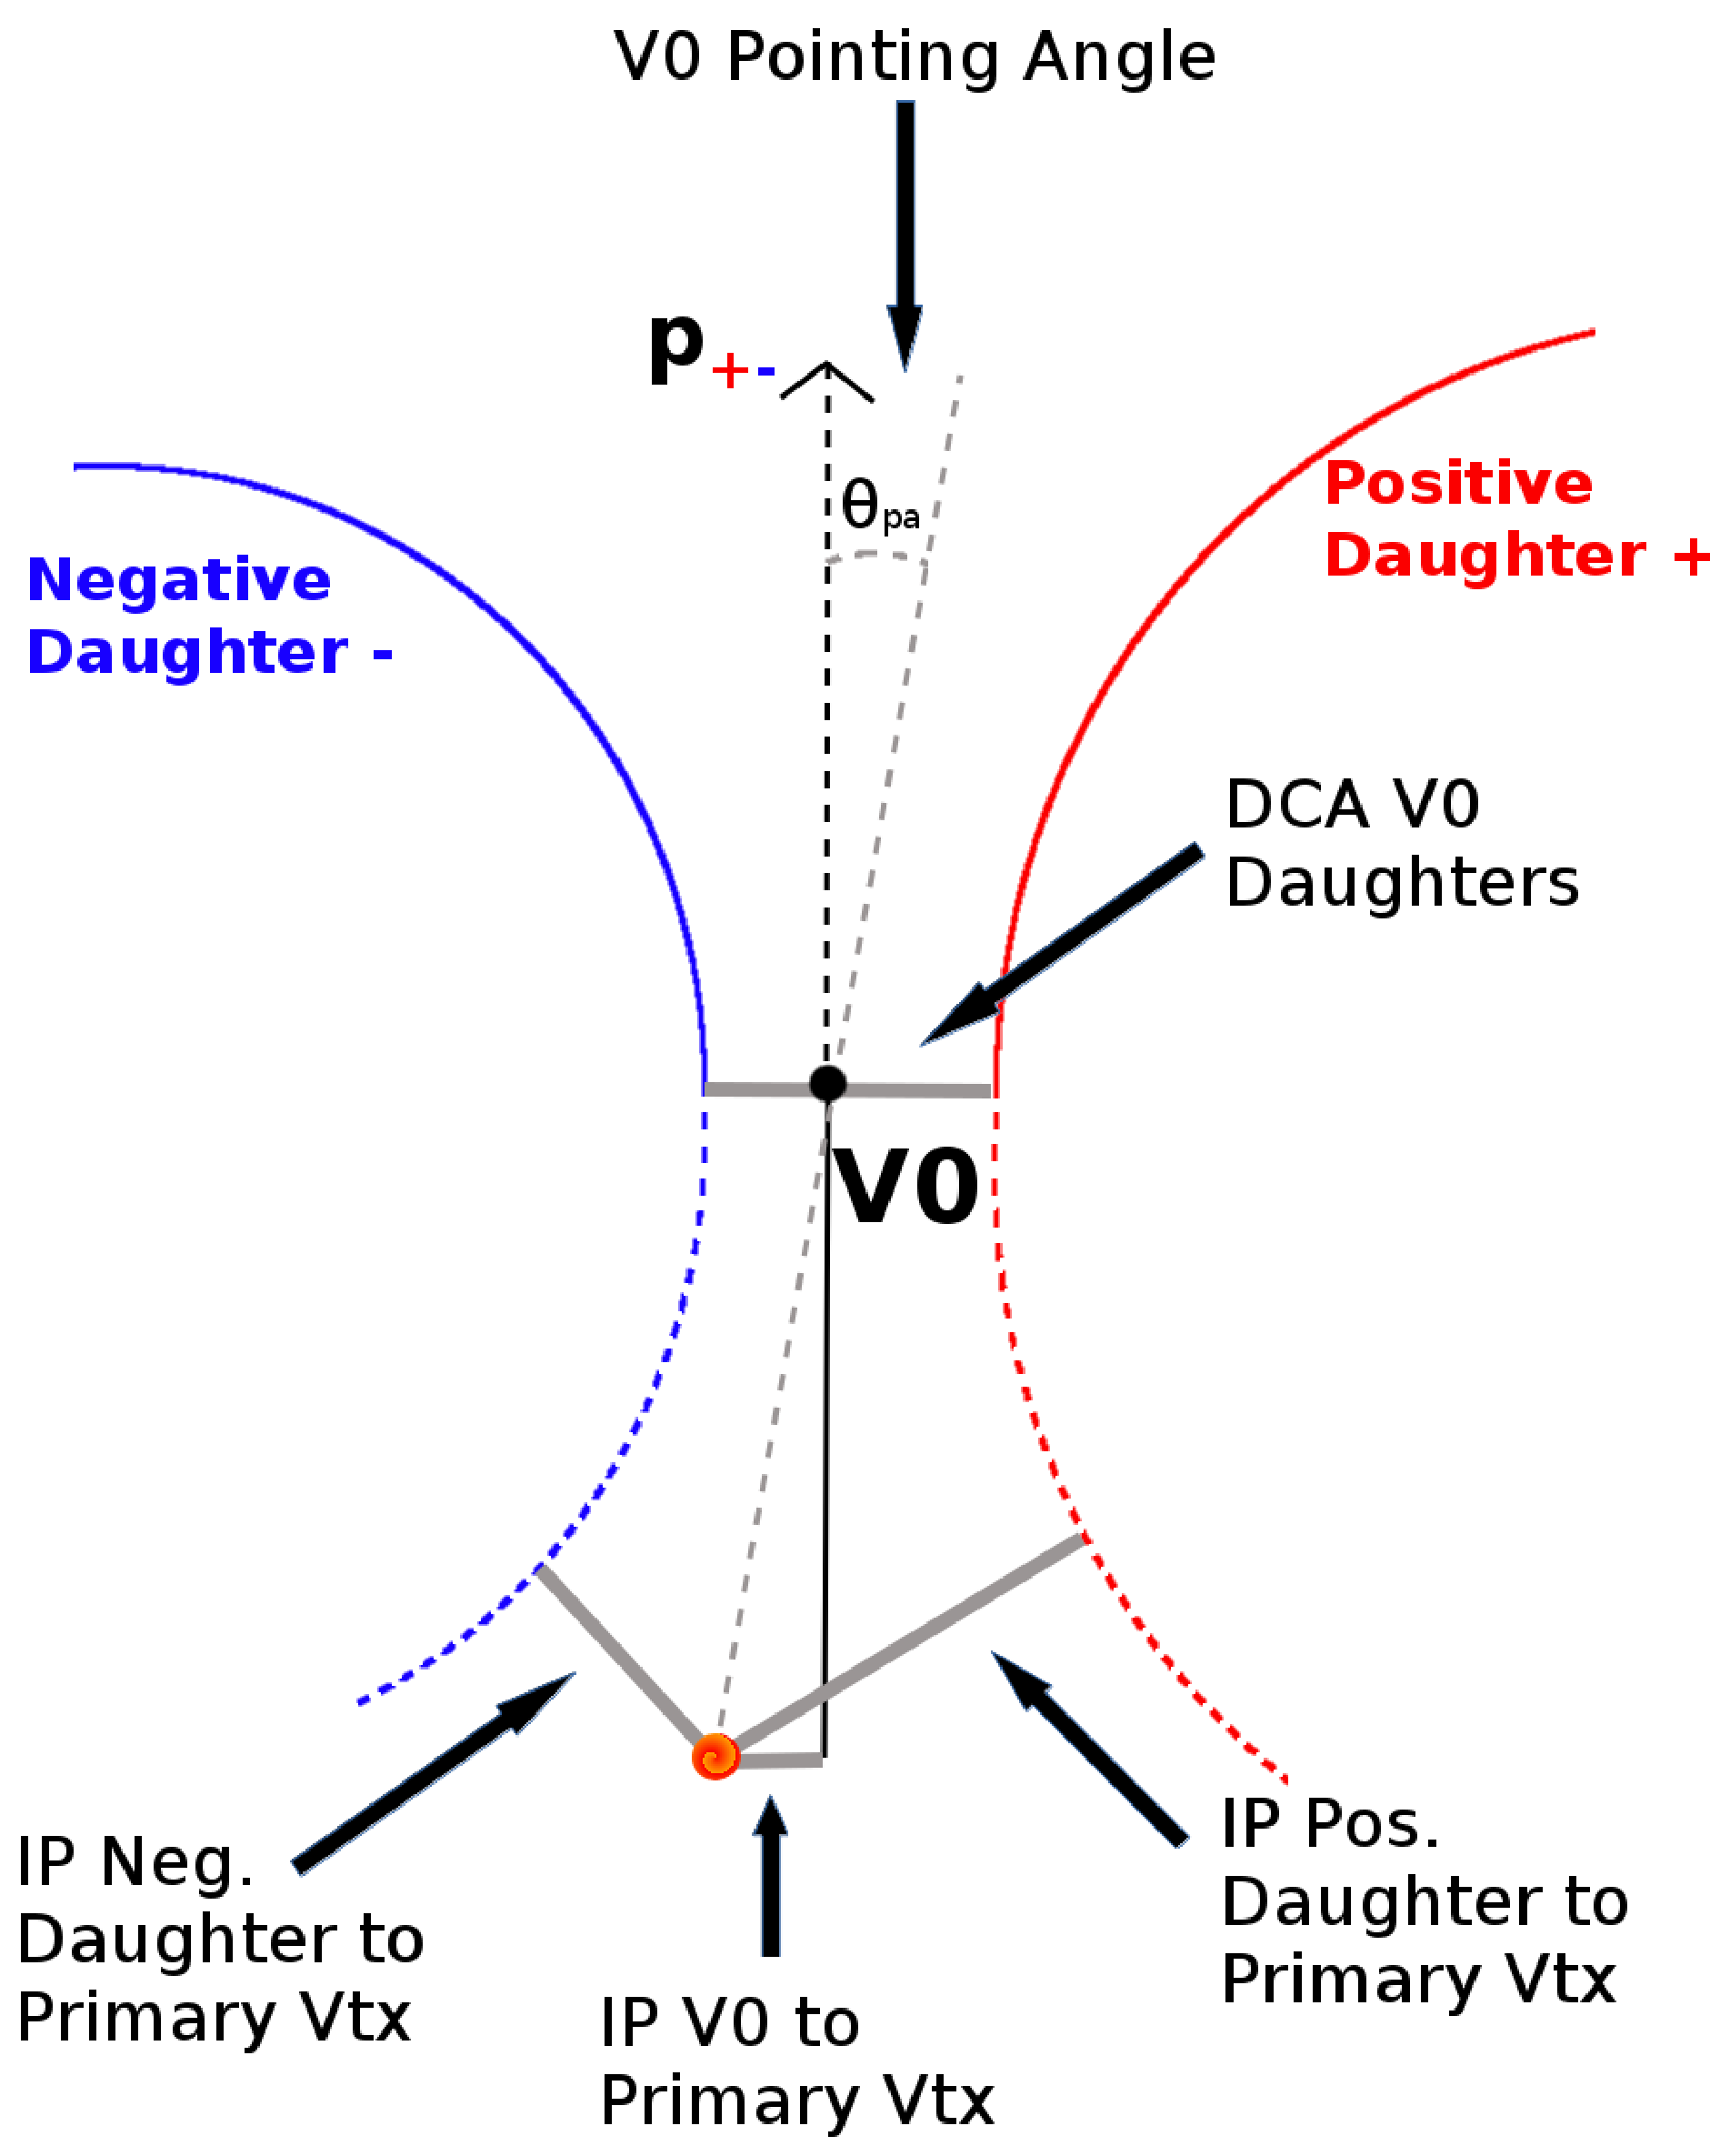
\includegraphics[width=0.9\linewidth]{3_DataSelection/Figures/V0CutsGeneral.pdf} 
  \caption[V0 Reconstruction]{V0 Reconstruction}
  \label{fig:V0Reconstruction}
\end{wrapfigure}
\end{comment}

\begin{figure}[h]
  \centering
  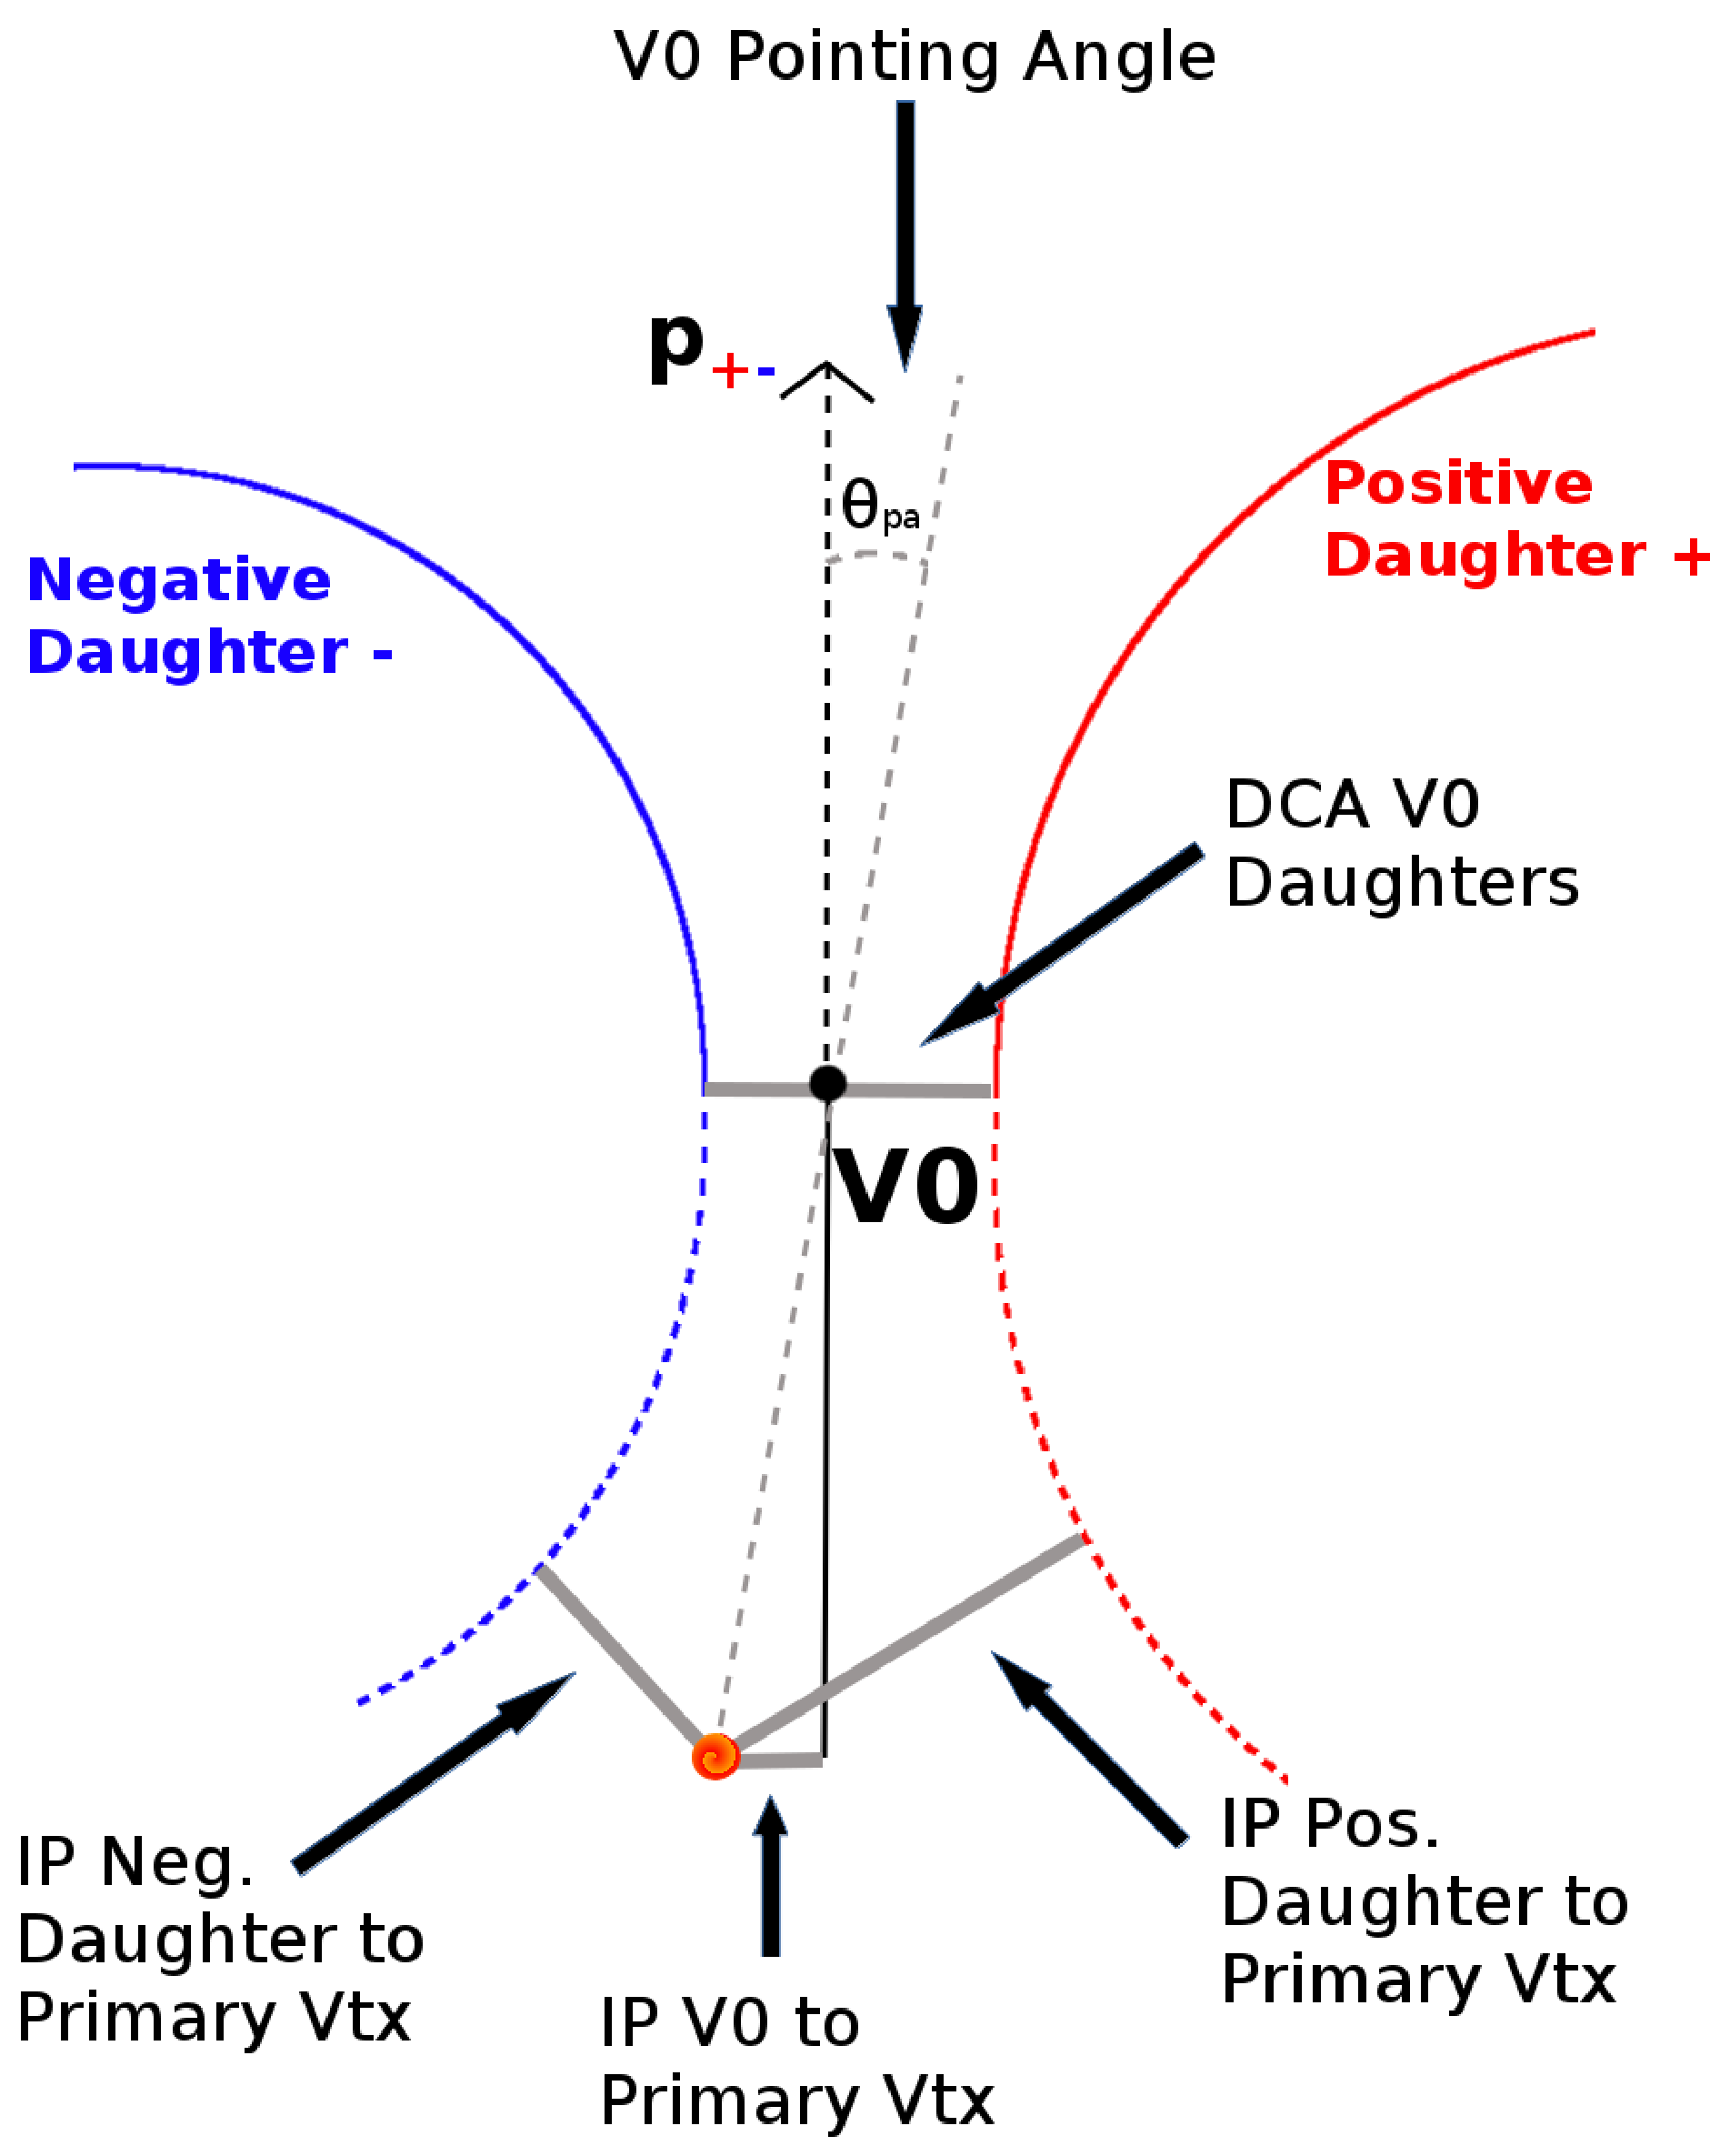
\includegraphics[width=0.5\textwidth]{3_DataSelection/Figures/V0CutsGeneral.pdf}
  \caption[V0 Reconstruction]{V0 Reconstruction}
  \label{fig:V0Reconstruction}
\end{figure}

To construct a V0 particle, the charged daughter tracks must first be found.  
Aside from typical kinematic and PID cuts (using TPC and TOF detectors), the daughter tracks are also exposed to a minimum cut on their impact parameter with respect to the primary vertex.  
The daughters of a V0 particle should not originate from the primary vertex, but rather from the decay vertex of the V0, hence the minimum cut imposition.  
The decay vertex of the V0 is assumed to be the point of closest approach between the daughter tracks.
To help ensure quality, a maximum value cut is demanded on the distance-of-closest-approach between the daughters (DCA V0 Daughters).
The positive and negative daughter tracks are combined to form the V0 candidate, the momentum of which is simply the sum of the momenta of the daughters (calculated at the DCA).

A minimum transverse momentum cut on the V0 candidate is introduced to reduce contamination from fake candidates.
Opposite to that of the daughter tracks, the V0 candidate is exposed to a maximum cut on its impact parameter with respect to the primary vertex.
In this case, we do want our V0 candidates to be primary, hence the maximum cut imposition.
To further strengthen our selection of primary V0 candidates, we impose a selection on the pointing angle, $\theta_{\mathrm{pa}}$, between the V0 momentum and the vector pointing from the primary vertex to the secondary V0 decay vertex.
We want the V0 candidate's momentum to point back to the primary decay vertex, and therefor a small $\theta_{\mathrm{pa}}$; we achieve this by appointing a minimum value on $\cos(\theta_{\mathrm{pa}})$ (``Cosine of pointing angle'' in Tables \ref{tab:LamCuts} and \ref{tab:K0sCuts}).

On occasion, \LamALam particles are misidentified as \Ks, and vice versa.  
To attempt to remove these contaminations without throwing away good candidates, we impose a set of misidentification cuts.  
The intent of these cuts is to judge whether a candidate is more likely a \LamALam or a \Ks, and are implemented as described below.  
For a given V0, we calculate the mass assuming different identities (\Lam, \ALam, \Ks) of the candidate; the mass assuming \Ks hypothesis ($m_{\mathrm{inv,~ K^{0}_{S}~ hyp.}}$) is calculated assuming $\pi^{+}\pi^{-}$ daughters, the mass assuming \Lam hypothesis ($m_{\mathrm{inv,~ \Lambda~ hyp.}}$) is calculated assuming p$\pi^{-}$ daughters, and the mass assuming \ALam hypothesis ($m_{\mathrm{inv,~ \bar{\Lambda}~ hyp.}}$) is calculated assuming $\bar{p}\pi^{+}$ daughters.  
In addition to the notation just introduced, in the following, $m_{\mathrm{PDG,~ K^{0}_{S}}}$ and $m_{\mathrm{PDG,~ \Lambda(\bar{\Lambda})}}$ denote the particle masses of the \Ks and \LamALam, respectively, as recorded by the Particle Data Group \cite{Patrignani:2016xqp}.

For \LamALam selection, a candidate is assumed to be misidentified and is rejected if all of the following criteria are satisfied:

\begin{enumerate}
 \item $\left|m_{\mathrm{inv,~ K^{0}_{S}~ hyp.}} - m_{\mathrm{PDG,~ K^{0}_{S}}}\right| < $ 9.0 MeV/c$^{2}$
 \item The daughter particles pass daughter cuts intended for \Ks reconstruction
 \begin{enumerate}
  \item \Lam selection
  \begin{enumerate}
   \item p daughter passes $\pi^{+}$ cuts intended for \Ks reconstruction
   \item $\pi^{-}$ daughter passes $\pi^{-}$ cuts intended for \Ks reconstruction.
  \end{enumerate}
  \item \ALam selection
  \begin{enumerate}
   \item $\pi^{+}$ daughter passes $\pi^{+}$ cuts intended for \Ks reconstruction
   \item $\bar{\mathrm{p}}$ daughter passes $\pi^{-}$ cuts intended for \Ks reconstruction.
  \end{enumerate}  
 \end{enumerate}
 \item $\left|m_{\mathrm{inv,~ K^{0}_{S}~ hyp.}} - m_{\mathrm{PDG,~ K^{0}_{S}}}\right|~ < ~\left|m_{\mathrm{inv,~ \Lambda(\bar{\Lambda})~ hyp.}} - m_{\mathrm{PDG,~ \Lambda(\bar{\Lambda})}}\right|$
\end{enumerate} 

Similarly, for \Ks selection, a candidate is rejected if all of the following criteria are satisfied for the \Lam case, or for the \ALam case:

\begin{enumerate}
 \item $\left|m_{\mathrm{inv}, \ \Lambda(\bar{\Lambda}) \ \mathrm{hyp.}} - m_{\mathrm{PDG},\ \Lambda(\bar{\Lambda})}\right| < $ 9.0 MeV/$c^{2}$
 \item The daughter particles pass daughter cuts intended for \LamALam reconstruction
 \begin{enumerate}
  \item $\pi^{+}$ daughter passes p($\pi^{+}$) daughter cut intended for \LamALam reconstruction
  \item $\pi^{-}$ daughter passes $\pi^{-}$($\bar{\mathrm{p}}$)
 \end{enumerate}
 \item $\left|m_{\mathrm{inv}, \ \Lambda(\bar{\Lambda}) \ \mathrm{hyp.}} - m_{\mathrm{PDG},\ \Lambda(\bar{\Lambda})}\right|~ < ~\left|m_{\mathrm{inv},~ \mathrm{K}^{0}_{S}~ \mathrm{hyp.}} - m_{\mathrm{PDG},~ \mathrm{K}^{0}_{S}}\right|$
\end{enumerate} 

At this stage, we have a collection of V0 candidates satisfying all of the aforementioned cuts.
However, this collection is still polluted by fake V0s, for which the daughter particles happen to pass all of our cuts, but which do not actually originate from a V0.
Although the two daughter particles appear to reconstruct a V0 candidate, they are lacking one critical requirement: the system invariant mass does not match that of our desired V0 species (these can be seen outside of the mass peaks in Fig. \ref{fig:Purities}).
Therefore, as our final single-particle cut, we require the invariant mass of the V0 candidate to fall within the mass peak of our desired species.
Note, however, that some fake V0s still make it past this final cut, as their invariant mass also happens to fall without our acceptance window.


Occasionally, we encounter a situation where two V0 candidates share a common daughter.
Not both of these candidates can be real V0s, and including both could introduce an artificial signal into our data.
To avoid any auto-correlation effects, for each event, we impose a single-particle shared daughter cut on each collection of V0 candidates.
This cut iterates through the V0 collection to ensure that no daughter is claimed by more than one V0 candidate.
If a shared daughter is found between two V0 candidates, that candidate with a smaller DCA to primary vertex is kept while the other is excluded from the analysis.
Note, this single-particle shared daughter cut is unique from the pair shared daughter cut discussed in Sec. \ref{PairSelection}, the latter of which ensure there is no daughter sharing between the particles in a given pair.

The specific cuts used to reconstruct our \LamALam and \Ks populations, along with plots showing the effect of the misidentification cuts, are shown in the following sections.

\subfile{3_DataSelection/3.3_V0Selection/3.3.1_LambdaReconstruction/3.3.1_LambdaReconstruction.tex}
\subfile{3_DataSelection/3.3_V0Selection/3.3.2_K0sReconstruction/3.3.2_K0sReconstruction.tex}
\subfile{3_DataSelection/3.3_V0Selection/3.3.3_V0PurityEstimation/3.3.3_V0PurityEstimation.tex}
\subfile{3_DataSelection/3.3_V0Selection/3.3.4_V0PurityBgdEstimator/3.3.4_V0PurityBgdEstimator.tex}

\end{document}
